\documentclass[twocolumn]{report}

\usepackage[utf8]{inputenc}
\usepackage[bottom]{footmisc}
\usepackage{amsmath}
\usepackage{float}
\usepackage{listings}
\usepackage{array}
\usepackage{algorithmic}
\usepackage{caption}
\usepackage{blkarray}
\usepackage{tabularx}

\usepackage[pdftex]{graphicx}
% declare the path(s) where your graphic files are
% \graphicspath{{../pdf/}{../jpeg/}}
% and their extensions so you won't have to specify these with
% every instance of \includegraphics
% \DeclareGraphicsExtensions{.pdf,.jpeg,.png}



% Title Page
\title{Lab 1 TBMI26 Neural Networks}
\author{Anton Sterner\\ antst719@student.liu.se\\ \\ Rasmus Ståhl\\ rasst403@student.liu.se\\ \\ Linköping University}

\begin{document}
	\maketitle
	
	\newpage
	\chapter{Supervised learning}
	
	\textbf{1. Give an overview of the data from a machine learning perspective. Consider if you need linear or non-linear classifiers etc.}
	
	
	Some of the datasets contain only two classes that are easily linearly separable. When data-samples are linearly separable, then one should use linear classifiers like kNN and Single-Layer Neural Networks. When the samples are not linearly separable then you you use non-linear classifiers like Multi-Layer Neural Networks. \\
	
	\textbf{2. Explain why the down sampling of the OCR data (done as pre-processing) result in a more robust feature representation.}
	
	Using downsampled data, the model is less prone to overfitting, making for a more generalized model. \\
	
	\textbf{3. Give a short summary of how you implemented the kNN algorithm.  }
	
	A training set (Xt) and a test set (X) of features is sent in as arguments to kNN.m along with the number of neighbors (k) and a matrix containing the class labels of the training set. The euclidean distances from each point in the training set to every point in the test set is calculated.  The distances are sorted in ascending order, and the k first elements from this vector are the k-nearest neighbors to that point. Then using Matlabs mode-function the most frequent class member is identified in this array, and the current sample in X is labeled as being a member of that class. This is repeated for all samples in X so that each test set sample gets classified. \\
	
	\textbf{4. Explain how you handle draws in kNN, e.g. with two classes (k = 2)?}
	
	In this case, the test sample is classified as a member of the class of the training sample that is has the smallest distance to. the mode function handles draws by simply returning the smallest of the values compared e.g. if class “1” and class “2” are at a draw, it will return “1”, as it is the smaller number. This could give a slight bias in the results, but it can be considered negligible for this application. 
	
	\textbf{5. Explain how you selected the best k for each dataset using cross validation. Include the accuracy and images of your results for each dataset.}
	
	We tested each dataset with different k values ranging from 1 to 50 and extracted the k value that gave the highest accuracy. Figure \ref{img:accuracy} is a plot of k-value versus accuracy. It can be seen that the first dataset can be classified correctly with 100 percent accuracy by this simple linear classifier. The other datasets are more complex, containing more classes and less clustered data points. The simple KNN-algorithm is not good enough for these datasets. Table 1 contains the best observed accuracy and k-value for each dataset. Note that these results can vary slightly depending on which points are selected as training and test data.  
	
	\begin{figure}
		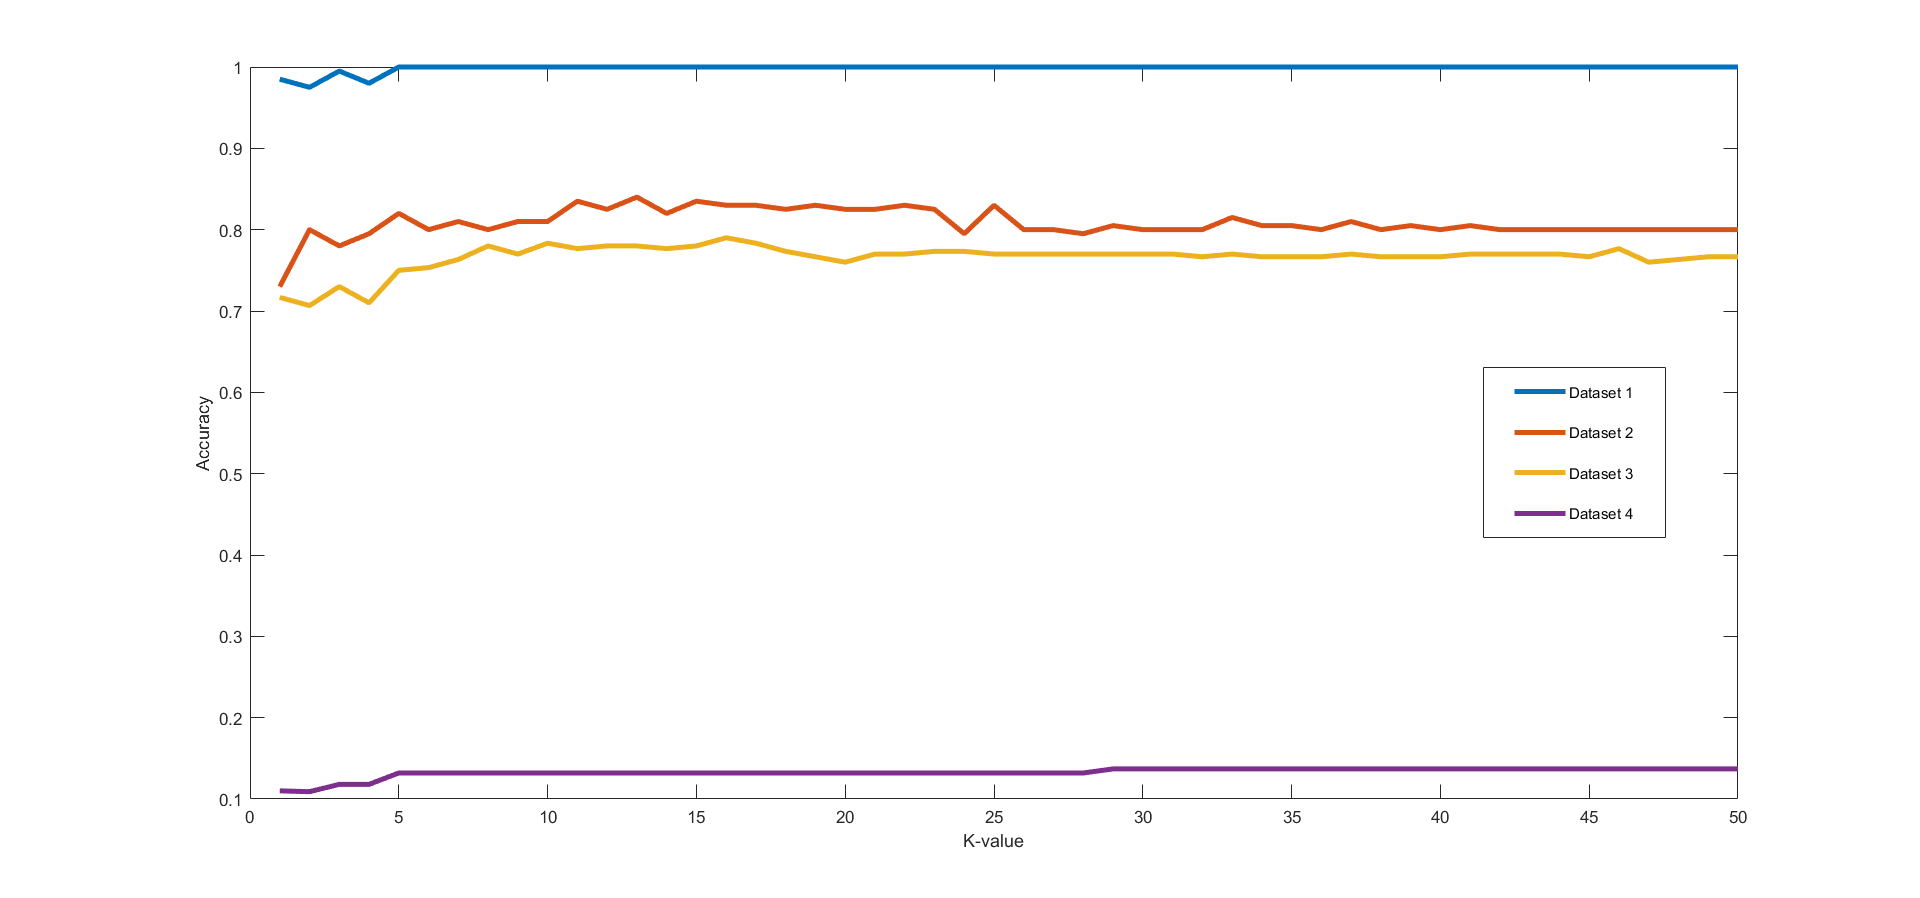
\includegraphics[width=8cm]{../accuracy2.png}
		\label{img:accuracy}
		\caption{K-value vs. accuracy for all four datasets.}
	\end{figure}
	
	\begin{table}
		\caption{Best accuracy and k-value for each dataset using K-NN classifier.}
		\centering
		\label{}
		\begin{tabular}{c|c|c|c|c}
			\hline
			\textbf{Dataset} & 1 & 2 & 3 & 4\\
			\hline
			\textbf{Best k-value} & 5 & 13 & 16 & 29\\
			\hline
			\textbf{Accuracy (\%)} & 100 & 84 & 79 & 13.4\\
			\hline
		\end{tabular} 
	\end{table}
	
	\textbf{6. Give a short summary of your backprop network implementations (single + multi). You do not need to derive the update rules.}
	A bias weight row is added to the training and test data as a preparatory measure for the computations. One vector containing weights is initialized with random numbers in the range -0.1 to 0.1 (two vectors for the multi-layer network). When training the networks, these weights are multiplied with the feature vectors to produce an output. If the output differs from the desired output of the model, the weights are adjusted by moving along the gradient, computed by the minimization algorithm. \\
	
	\textbf{7. Present the results from the backprop training and how you reached the accuracy criteria for each dataset. Motivate your choice of network for each dataset. Explain how you selected good values for the learning rate, iterations and number of hidden neurons. Include images of your best result for each dataset, including parameters etc.}
	
	Dataset 1 is the simplest set with clear clusters of points, and can be solved with good accuracy using the single layer network. The single layer network does not perform very well with datasets 2-4, for those sets the multi-layer network is used. Table 2 shows the gathered results for all datasets using the two neural network classifiers. 
	
	The classification of test samples for dataset 1 is shown in figure 2. Only one of 200 points are classified wrongly using this linear decision boundary. 
	
	In the training of these classifiers, the accuracy in classification of the test samples are generally better when not all available samples are used for training the model (downsampling of data). This makes for a more generalized model as described before. \\
	
	\begin{table}[t]
		\caption{Results of training single-layer and multi-layer neural networks for the different datasets.} 
		\label{tab:title} 
		\centering
		\begin{tabular}{|c|c|c|c|c|}
			\hline
			\textbf{Dataset} & 1 & 2 & 3 & 4\\
			\hline
			\textbf{Network} & Single-layer & Multi-layer & Multi-layer & Multi-layer\\
			\hline
			\textbf{Number of hidden units} & 0 & 5 & 10 & 50\\
			\hline
			\textbf{Iterations} & 5000 & 20000 & 20000 & 13000\\
			\hline
			\textbf{Learning rate} & 0.001 & 0.005 & 0.005 & 0.01\\
			\hline
			\textbf{Accuracy (\%)} & 99.5 & 99.5 & 99.667 & 96.606\\
			\hline
		\end{tabular} 
	\end{table}
	
	\begin{figure}[h]
		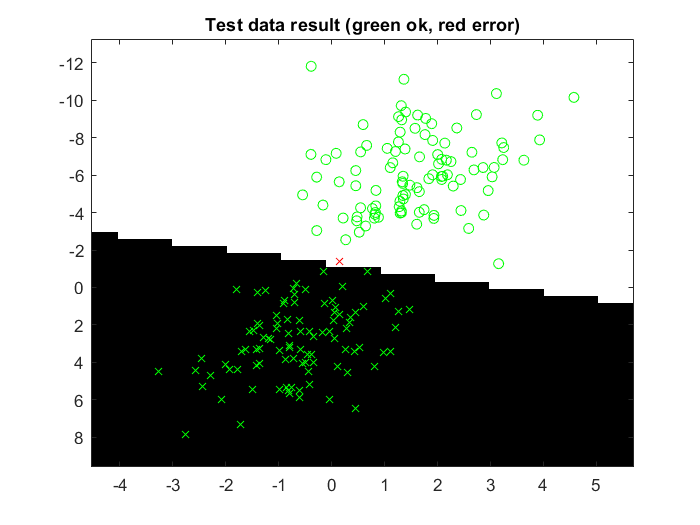
\includegraphics[width=8cm]{../single_set1.png}
		\label{img:testset1}
		\caption{Test data results for dataset 1. Single-layer network.}
	\end{figure}
	
	\begin{figure}[h]
		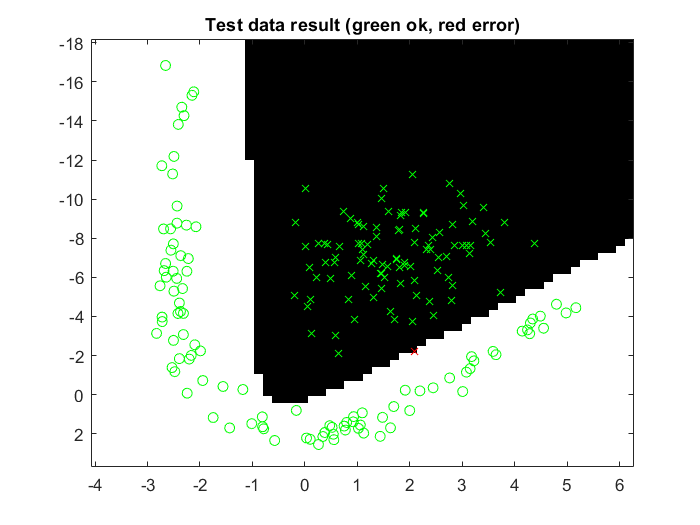
\includegraphics[width=8cm]{../multi_set2.png}
		\label{img:testset1}
		\caption{Test data results for dataset 2. Multi-layer network.}
	\end{figure}
	
	\begin{figure}[h]
		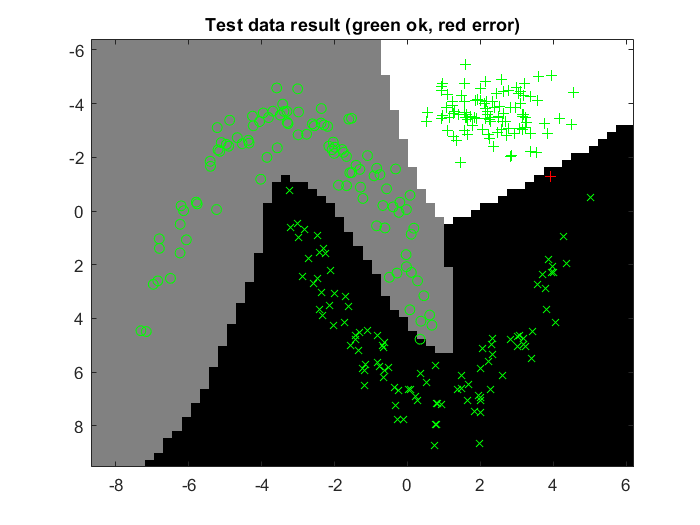
\includegraphics[width=8cm]{../multi_set3.png}
		\label{img:testset1}
		\caption{Test data results for dataset 3. Multi-layer network.}
	\end{figure}
	
	\textbf{8. Present the results, including images, of your example of a non-generalizable backprop solution. Explain why this example is non-generalizable.}
	To create a non-generalizable solution, the number of training samples are greatly 	reduced, while testing the model with all available samples. The figures 5-7 shows the error of the model using training and test data, and the classified samples using training and test data. When training with few samples, the model does not adjust well to the distribition of points in the full data set. In this case the multi-layer network is used, but only with 2 hidden units. The accuracy of classification is still 74 percent, which is good considering the very limited number of training points. \\
	
	\begin{figure}
		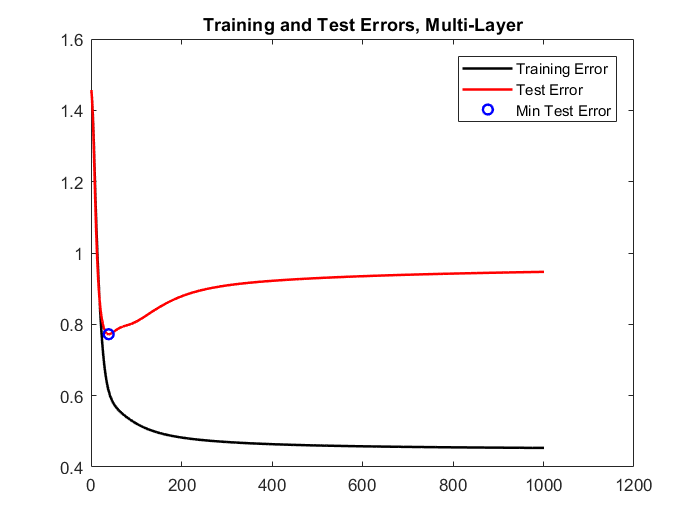
\includegraphics[width=8cm]{../error_set3.png}
		\label{img:testset1}
		\caption{Training and test errors for dataset 3. Multi-layer network.}
	\end{figure}
	
	\begin{figure}
		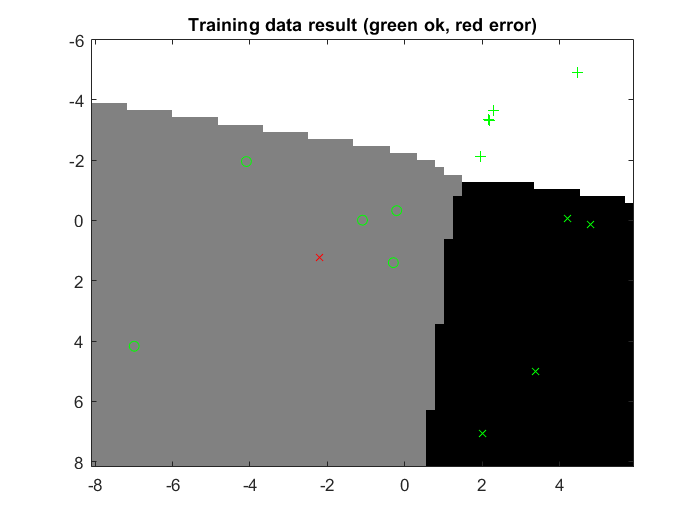
\includegraphics[width=8cm]{../training_set3.png}
		\label{img:testset1}
		\caption{Training data result.}
	\end{figure}
	
	\begin{figure}
		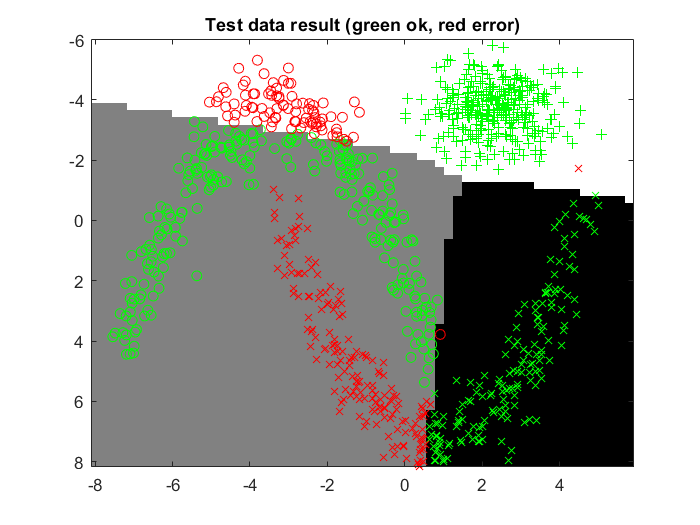
\includegraphics[width=8cm]{../test_set3.png}
		\label{img:testset1}
		\caption{Test data result.}
	\end{figure}
	
	\textbf{9.Give a final discussion and conclusion where you explain the differences between the performances of the different classifiers. Pros and cons etc. }
	
	The single-layered network can clearly handle linearly separable datasets, and is the best choice when using dataset 1 over a multi-layered network which is more computationally expensive. But when it comes to datasets which are not linearly separable a multi-layered network is needed, using a nonlinear activation function providing nonlinear mapping. Dataset 4 is the best example of this, using a hidden layer with many units, 50 in this case, is the only way of getting an accuracy over 96 percent. \\
	
	\textbf{10. Do you think there is something that can improve the results? Pre-processing, algorithm-wise etc.}
	
	You could add a momentum term which adjusts the step size towards local minima when optimizing. This will help the optimization algorithm in avoiding suboptimal solutions, and thereby improve the chances of correct classifications.
	
\end{document}          

